\documentclass[journal]{IEEEtran}

\renewcommand\thesection{\arabic{section}} 
\renewcommand\thesubsectiondis{\thesection.\arabic{subsection}}
\renewcommand\thesubsubsectiondis{\thesubsectiondis.\alph{subsubsection}}
\renewcommand\theparagraphdis{\arabic{paragraph}.}

%\usepackage[retainorgcmds]{IEEEtrantools}
%\usepackage{bibentry}  
\usepackage{xcolor,soul,framed} %,caption

\colorlet{shadecolor}{yellow}
% \usepackage{color,soul}
\usepackage[pdftex]{graphicx}
\usepackage[cmex10]{amsmath}
\usepackage{array}
\usepackage{mdwmath}
\usepackage{mdwtab}
\usepackage{eqparbox}
\usepackage{url}
\usepackage{amsfonts}
\hyphenation{op-tical net-works semi-conduc-tor}
\usepackage{graphicx}

\usepackage{xcolor}
\definecolor{th}{RGB}{0,83,161}
\graphicspath{{../pdf/}{../jpeg/}}
\DeclareGraphicsExtensions{.pdf,.jpeg,.png}

\usepackage[
    bookmarks=true,
    bookmarksopen=true,
    bookmarksnumbered=true,
    bookmarksopenlevel=1,
    pdfpagelabels=true,
    colorlinks=true,
    linkcolor=th,
    urlcolor=magenta,
    anchorcolor=black,
    citecolor=cyan,
    filecolor=magenta,
    menucolor=red,
    plainpages=false,
    hypertexnames=true,
    linktocpage=false,
]{hyperref}

\usepackage[cmex10]{amsmath}
%Mathabx do not work on ScribTex => Removed
%\usepackage{mathabx}
\usepackage{array}
\usepackage{mdwmath}
\usepackage{mdwtab}
\usepackage{eqparbox}
\usepackage{url}
\hyphenation{op-tical net-works semi-conduc-tor}
\usepackage{graphicx}



%\bstctlcite{IEEE:BSTcontrol}
%=== TITLE & AUTHORS ====================================================================
\begin{document}

\bstctlcite{IEEEexample:BSTcontrol}
	
    \title{    
    
\includegraphics[width=4.5in]{photo/logo.png}
    \newline \newline
     IT-Projekt \\ 
     \textit{Autonmously driving Remote Control Car}
     }

  \author{
      \textbf{L\"OHR} Tim,
      \textbf{BOHNSTEDT} Timo, 
      \textbf{PALPANES} Ioannis
}

% The paper headers
\markboth{IT-Project at the TH-OHM
}{Roberg \MakeLowercase{\textit{et al.}}}


% ====================================================================
\maketitle
% === ABSTRACT 
\begin{abstract}
Im Rahmen unseres IT-Projekts beschäftigen wir uns mit der Entwicklung eines autonom fahrendes ferngesteuertes Auto. 
ToDo
\end{abstract}

% === KEYWORDS 
\begin{IEEEkeywords}
\hl{Machine Learning, IT-Project, RC-Car, RaspberryPi, Autonomusly driving}
\end{IEEEkeywords}
\IEEEpeerreviewmaketitle

% === I. Project background and motivation
\section{Project background and motivation}
ToDo

\section{Literature Survey}
\label{sec:LiteratureSurvey}
\subsection{Reinforcement Learning}

\section{Hardware}
\subsection{RC Car}
<<<<<<< HEAD
Our car is the \textit{s-idee® 18175 9115 RC Car Buggy waterproof monstertruck 1:12}.
The remote control car is the heart of our project. Eventhough basically every remote control car can be used to drive autonomously, it is a better choice to buy a real model car, because a real servomotor makes it much easier. The cost of a real model RC car is approximately 100 euros. It is neccessary that the car is quite large, because we need to store the Raspberry Pi, the camera and a powerbank for the Pi onto the car. To keep everything in position, we attached it with a 3D print of a holding system, which was tailored by us for our car. \\

\subsubsection{Technical Details}
Our car comes with 2,4 GHz type of the remote control and is 40 km/h fast. It only weights 1,88 Kg. Since the car is normaled steered by the remote control, in our case we use the Raspberry Pi to drive it autonomously. The battery is a 9,6V with 800 mah, which gives us plenty of time to capture pictures of the track to train the model on. The car like casing is easy to remove, to attach the Raspberry Pi and the rest onto it.

\subsubsection{Servomotor}

The servomotor is the key to connect the Raspberry Pi with the RC car. A normal servomotor has 2 times 3 pins connect to it. One responsible for the steering and the other one for the speed. The steering is managed by a so-called PWM (Pulse Width Modulation) as shown in figure \ref{pwm}. Depending on the length of the signal, the steering performs a certain degree of changing its ankle. We need to configure and setup the optimum values for our car in the Python \textit{steering} file. \\

\begin{figure}
  \begin{center}
  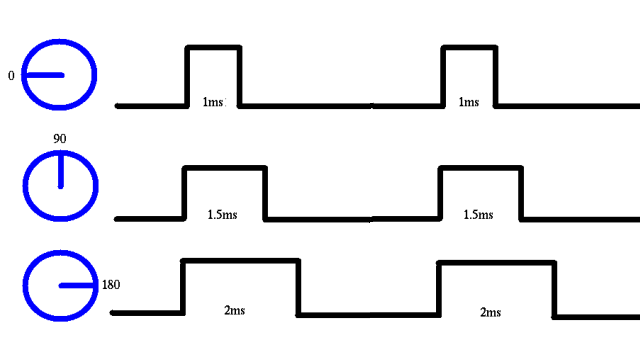
\includegraphics[width=2.5in]{photo/pwm}\\
  \caption{PWM signal}\label{pwm}
  \end{center}
\end{figure}

\subsection{Raspberry Pi}
Even though by now the Raspberry Pi 4 is out, we still use the Raspberry Pi 3B+, because we are sure that it is compatible with our other microcontrollers and software. \\
We use a 16GB SanDisc to store the operating system and the machine learning model on the Raspberry Pi. \\

\subsubsection{Technical Details}
The Raspberry Pi 3B+ is equipped with a lot of different extensions. It has a Wi-Fi module to communicate with the Python webserver and a farely fast processor to run the neural network and classify where to drive next. The Processor is the Broadcom BCM2837B0, Cortex-A53 with 1.4GHz and it has 1GB LPDDR2 SDRAM. \\
Furthermore for the connectivity the Pi has extended 40-pin GPIO headers. The weight is only 42 gramms, which makes it easy to attach it onto the RC car. The \textit{Donkey Car Project} \cite{donkey} provides a prepared operating system for the Raspberry Pi called \textit{donkeypi}. This OS is based on the basic \textit{raspbian OS} from the Raspberry Pi company, but also includes the prepared Python files to start the webserver, read in the images and drive autonomously based on the images classified through the trained model. \\

\subsubsection{Cameramodule}
For our purpose we use the Raspberry Pi Camera Module 8MP v2.1. It can capture pictures with 1080p and 8 megapixel focus. We are not required to use a wider lense, because our test track is big enough. The images captured by this camera are respectively the input for the model to train with. 1080p is fairely large and would take an eternity to train, this is why we need to scale the image down to 160x120 pixels. Furthermore we use a framerate of 20, which means we capture 20 images per second.  

\subsection{Servodriver}
We use the SunFounder PCA9685. The price for this microcontroller is approximatetly 13 euro on the most famous marketplaces. The servodriver is needed to produce the PWM (Pulse width modulation) signals for our Raspberry Pi. It acts as joint for the RC cars's servomotor and the Raspberry Pi. \\

=======
\subsubsection{Technischer Aufbau}
\subsubsection{Servomotor}

\subsection{Raspberry Pi}
\subsubsection{Technical Details}
\subsubsection{Cameramodule}

\subsection{Servodriver}
>>>>>>> b61d346bb0d98c19f46ea923086a7cd8e571eeb5
\subsubsection{Technical Details}

\subsection{Cable Management}

\section{Software Architecture}

In this section we give a quick overview in how the entire software is connected to each other (Figure \ref{webserver}).

\subsection{Python Files}

Since our group project is based on the \textit{Donkey Self-Driving Car} \cite{donkey} Project,  we are constraint to use the same folder structure. The main structure is:

\begin{itemize}
\item management
\item parts
\item templates
\item test
\end{itemize}

whereas management includes everything related to the webserver (as explained in the next subsection). The parts folder contains all the single devices related to get the car to drive by itself. Included in the parts folder is e.g. Pi Camera module, the keras neural network and the image configurations to use them as input for the neural network. 

\subsection{Webserver}

For the webserver we use the Python \textit{package} called \textit{Tornado}. Tornado is a basic multi purpose websocket which is open-source to use. It can be used for the bidirectional communication between the server and the browser. To receive the live transmission of the pictures of the camera module, we use the Tornado webserver. As shown in figure \ref{ebene2}, we access the webserver over the \textit{localhost} and the \textit{Port 37}. This Port is standardized by IEEE \footnote{\url{https://de.wikipedia.org/wiki/Liste_der_standardisierten_Ports}} as the \textit{TIME Protocol} and fits perfect to our requirements for tracking time intervalls.

\begin{figure}
  \begin{center}
  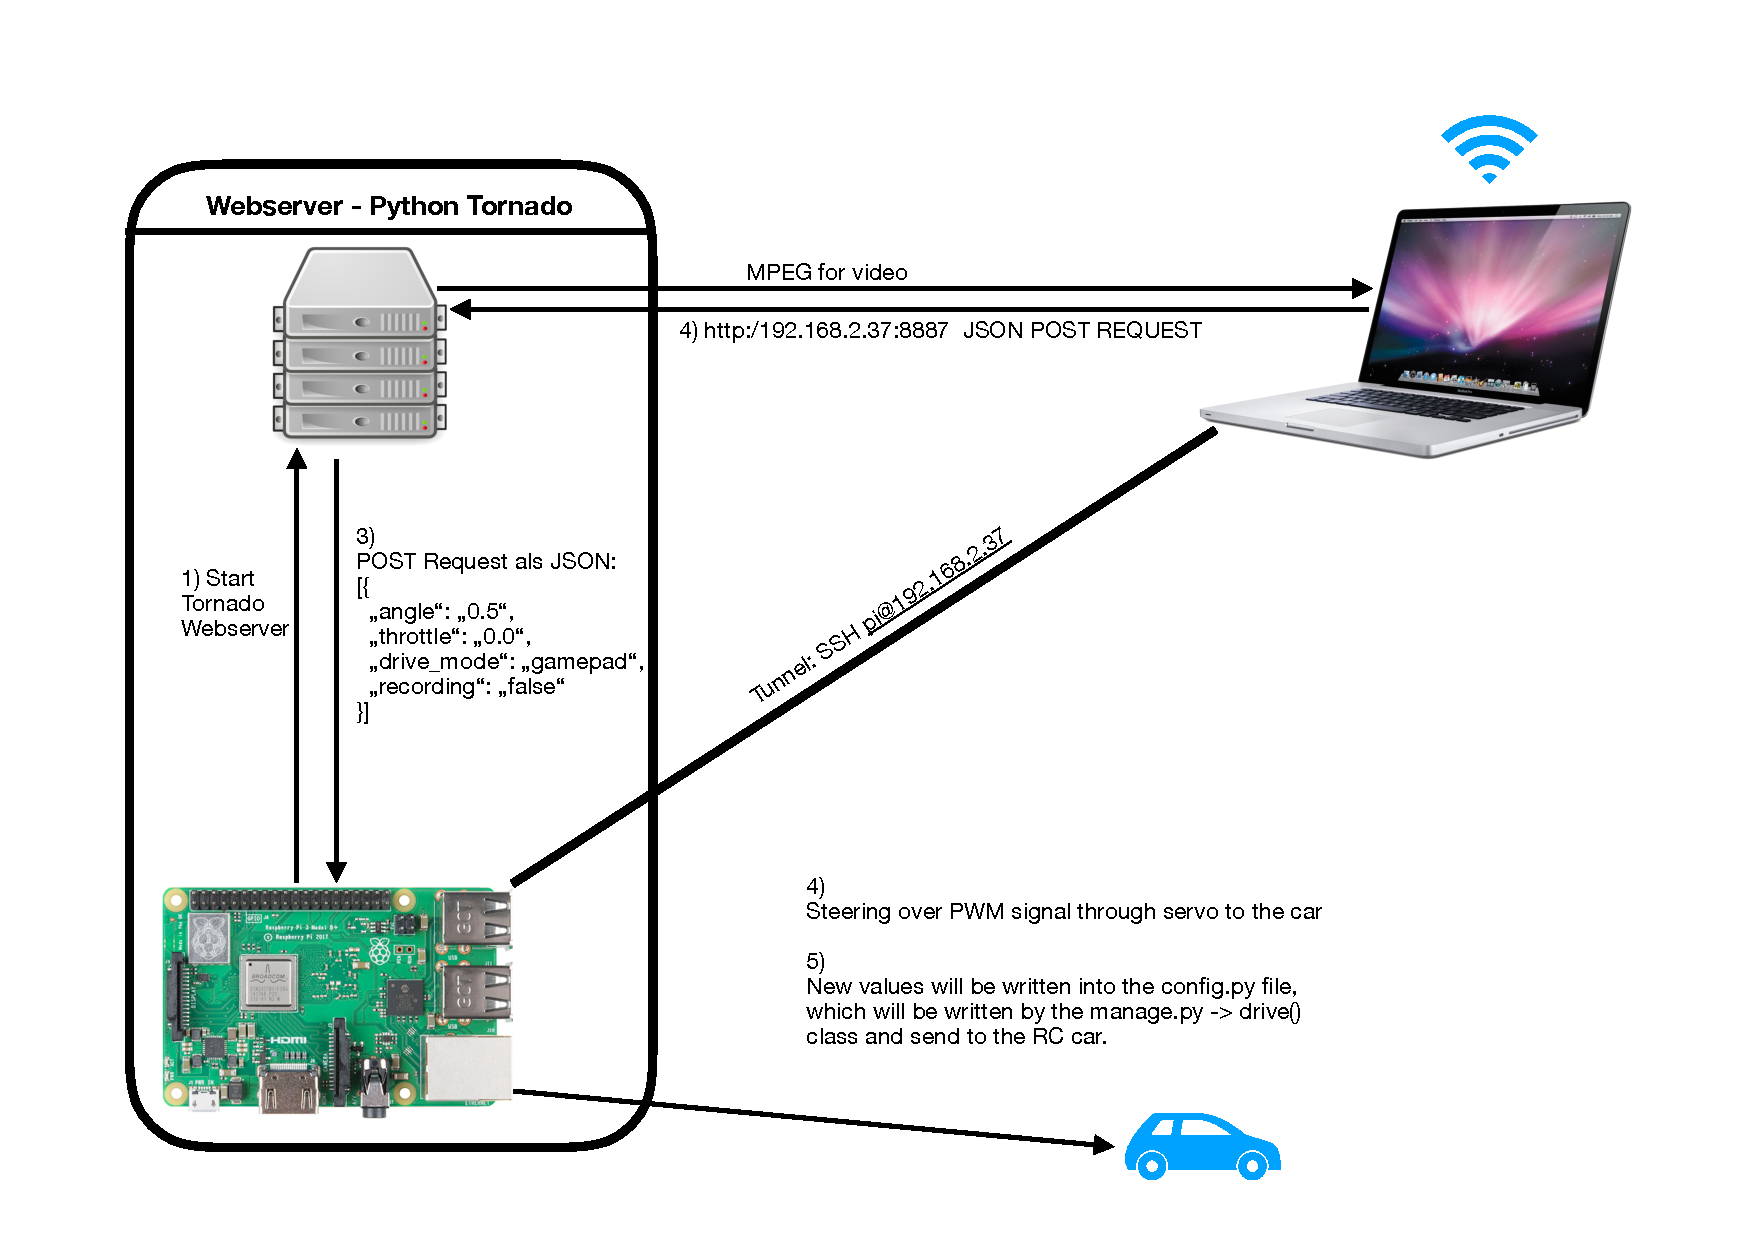
\includegraphics[width=3.5in]{photo/webserver.pdf}\\
  \caption{Webserver Overview}\label{webserver}
  \end{center}
\end{figure}

\subsection{Unity}

ToDo

\section{Deep Learning}
\noindent To solve the image classification task, we are using a convolutional neuronal network (CNN). CNN's are a particular case of feed-forward neural networks \cite{Goodfellow-et-al-2016}. On a very fundamental level, we can say that a feed-forward neural network - as the most machine learning models - is a function \cite{RN5}. The function of a feed-forward neural network can simply be described as \(y = f(x, \o )\) . CNN's and feed-forward neural networks are estimating parameter values. So for \(y = f(x, \o )\) we estimate the parameter \(\o \) \cite{Goodfellow-et-al-2016}. Through those estimated parameter values we are receiving a function back with the smallest possible difference between the predicted output values and the defined output values. A function that measures the difference between the expected - and the defined output is a so-called loss function \cite{Goodfellow-et-al-2016}. To compare our model accuracy with other model, we are using the following evaluation criteria:
\begin{equation}
Acc(f,D) = \frac{1}{m}\sum_{m}^{i=1} \mathbb{I} \left [ y^{(i)} =f(x^{()i)})\right ]
\label{acc}
\end{equation}
CNN's and classical feed-forward neuronal networks differ in their basis of calculation. Feed-forward neural networks are using matrix multiplication, whereas CNN's are using convolutions. Convolutional layers, pooling layers, and fully-connected layers are specific layers for a CNN \cite{LeCun1998}. \\

\subsubsection{Model Architecture}
\label{subsec:ModelArchitecture}
For our model, we choose pretty much the underlying implementation of the official website. It is an implementation of an architecture which is introduced by a group of researches which working for Nvidia. Their study showed that it is possible to train a model which can be used for autonomous driving. Especially the researchers showed that they are using a small amount of labelled data — more preseily,   only a few pictures from a short time of driving, where the images are marked with the direction in which the vehicle should drive\cite{LearningForSelf-DrivingCars}. As in our \hyperref[sec:LiteratureSurvey]{Literature Survey} mentioned Christian Friedrich Coors implemented the model before.  As he said, the model has 266.628 parameters which can be trained \cite{Coors}. The architecture u can see in Figure \ref{fig:Archi}.

\begin{figure}
  \begin{center}
  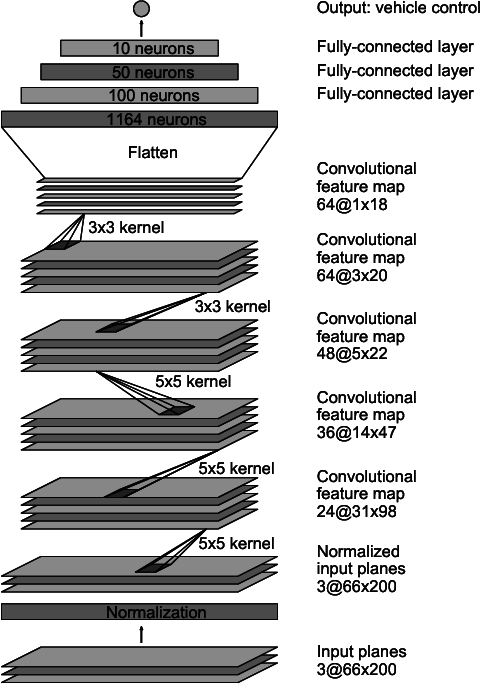
\includegraphics[width=3in]{photo/CNNArchitecture.png}\\
  \caption{Model Architecure from the Nvidia Research Team \cite{LearningForSelf-DrivingCars}}\label{featuremap}
  \label{fig:Archi}
  \end{center}
\end{figure}

The Team around Nvidia concluded in their paper that there is more work to do for getting the driving process more stable \cite{LearningForSelf-DrivingCars}. Jelena Kocić and their team focused on this task and got a better result. They reached their goal by using other building blocks like a pooling layer. They mentioned that the training process and the driving process is more computational intense. Because of our small hardware resources at the raspberry pi is why we decided to use the first model. \cite{AutomotivePlatformsAutonomousDriving}
\subsubsection{Convolutional Layers}
\noindent The convolutional Layer performs the extracting of features from the input matrix into a feature map. For this procedure, we use matrix multiplication in the form of the dot product and a filter (feature detector, kernel) \cite{Goodfellow-et-al-2016}. 

\begin{figure}
  \begin{center}
  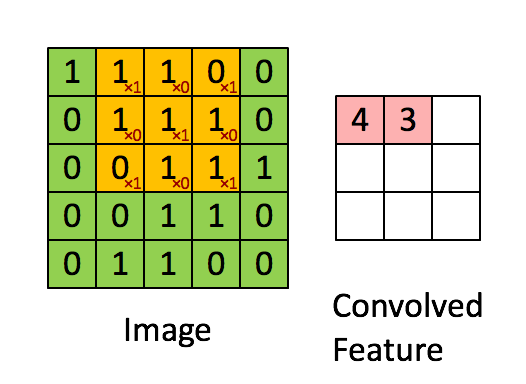
\includegraphics[width=3in]{photo/cnn.png}\\
  \caption{Feature Map derived from http://deeplearning.stanford.edu}\label{featuremap}
  \end{center}
\end{figure}

In picture \ref{featuremap} can be seen a calculation example of how convolution is applied to a matrix. We are iterating with the filter over the matrix, calculating the scalar product and writing the result into a feature map. An activation function like the rectified linear unit (ReLU) normalizes the feature map after we performed the convolution. Normalization guarantees a feature map which is not a linear transformation of its input value. If this is the case, we only have a linear problem which can be easily solved, but with a wrong results. In other words, the input values get just multiplied by coefficients. Note that there are plenty of reasons for activation functions in a neuronal network. We are giving a closer look at this topic at our section \hyperref[sec:activationFunctions]{"Activation Functions"}. In Figure \ref{featuremap1} you can see how our pictures had changed after applying the first convolutional layer, before and after doing normalization.  \\

\begin{figure}
  \begin{center}
  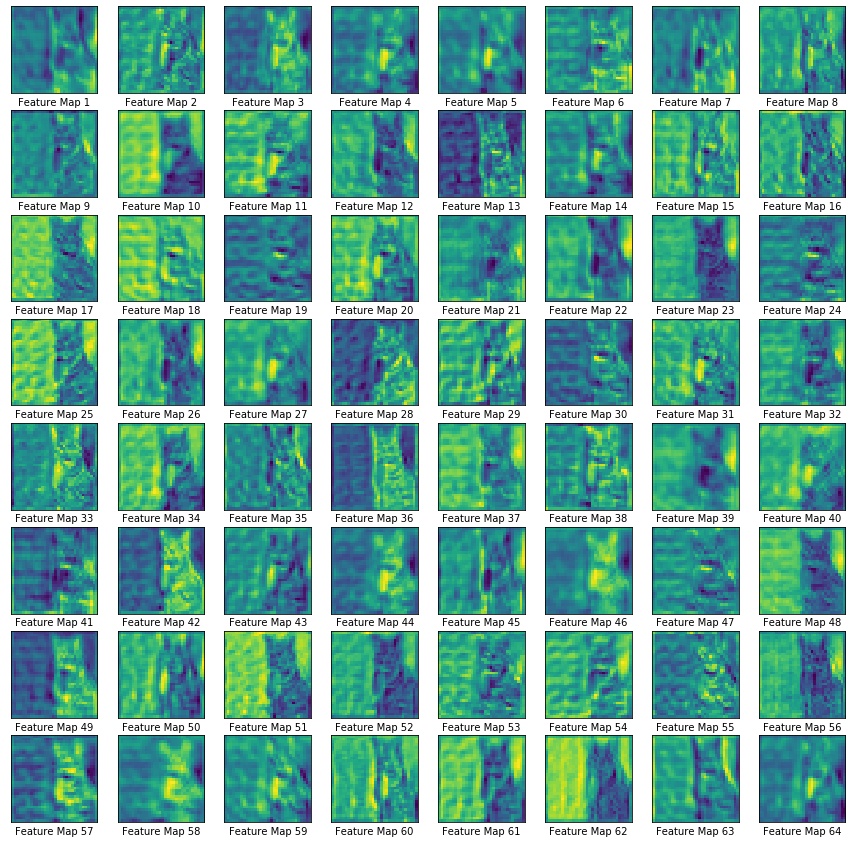
\includegraphics[width=3in]{photo/feature_map1.png}\\
  \caption{Feature Map from CNN Layer 1}\label{featuremap1}
  \end{center}
\end{figure}

\begin{figure}
  \begin{center}
  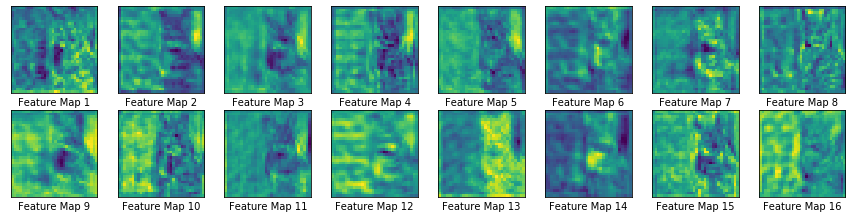
\includegraphics[width=3in]{photo/feature_map2.png}\\
  \caption{Feature Map from CNN Layer 2}\label{featuremap2}
  \end{center}
\end{figure}

This represents the 64 first feature maps of a random picture from the dataset. We can observe that the filters already focus on certain points on the cat's body. We further used this feature map as input for the second CNN layer. The output of the second feature map (figure \ref{featuremap2}) further sharpens the filters. For example we can see that feature map 2 until 5 focuses on the cat itself, whereas map 8 puts its focus on the cats ears. \\

\subsubsection{Pooling Layers}
\noindent It is common to add a pooling layer in-between the convolutional layers periodically. The function exists to avoid overfitting and step by step reduce the size of the input image by reducing the number of parameters and computations of the network \cite{RN2}. Anyways as mentioned earlier we decided against pooling layers as discussed in our \hyperref[subsec:ModelArchitecture]{Model Architecture} Section.\\
\subsubsection{Fully-Connected Layers}
\noindent The Dense layer is the last layer of our model. It is also called the \textit{fully connected layer}. Neurons in the fully connected layer have full connections to all activations in the previous layer, as in the normal neural networks. Their activation functions will then be computed by a matrix multiplication which is followed by a bias offset. 
For the ten different animals we respectively have ten fully connected neurons in the dense layer. \\
\subsubsection{Kernel Regularization}
\noindent There are many different regularizations to prevent the neural network from overfitting. For our project we chose the \textit{L2 regularization} because it is the most common form.
It can be integrated by penalizing the squared magnitude of all parameters directly in the objective. So, for every weight \textit{w} in the network, the term \(\frac{1}{2} \lambda w^2\) gets added to the objective, where \(\lambda \) is the regularization strength. It's usual to see \(\frac{1}{2}\) in the front, because the gradient of this term with respect to \textit{w} is simply \(\lambda w\) instead of \(2 \lambda w\). The L2 penalizes the peaky weight vectors and prefers the diffuse weight vectors \cite{RN4}. During the gradient descent weight update, the L2 regularization has the meaning, that every weight is decayed linearly (\textit{w += -lambda * w}) towards zero. \\
\subsubsection{Batch Normalization}
\noindent A technique developed by Ioffe and Szegedy \cite{RN4} is called Batch Normalization properly initializes neural networks by explicitly forcing the activations throughout a network to take on a unit gaussian distribution at the beginning of the training. Normalization is a simple differentiable operation. 
It allows to use higher learning rates at the beginning and is less vulnerable to a bad initialization. In other words, neural networks that implement batch normalization layers are significantly more robust. Additionally, batch normalization can be interpreted as a preprocessing step on every layer of the network. Batch normalization yields in general, a substantial improvement in the training process. \\
\subsubsection{Activation Functions}
\label{sec:activationFunctions}
\noindent There a couple of widely used activation functions like tanh, sigmoid function, ReLU or the ELU. For our model we decided to use the \textit{ReLU} activation function. The Rectified Linear Unit (ReLU) has become very popular in the last few years. It computes the function \(f(x)=max(0,x)\). In other words, the activation is simply thresholded at zero. There are plenty of pro's and con's for the ReLU:
\begin{itemize}
\item (+) Compared to tanh/sigmoid neurons that need to compute expensive operations  like the exponentials, the ReLU can be implemented by directly thresholding a matrix of activations at zero.
\item (+) It was found to notably accelerate the convergence of stochastic gradient descent (SGD) compared to the tanh/sigmoid functions. That is, because of its linear, non-saturating form.
\item (-) Sadly, ReLU units can be weak during training and possibly “die”. For example, a large gradient streaming through a ReLU neuron could cause the weights to update in a dead end, so that it will never activate again. If this happens, then the gradient streaming through the unit will forever be zero. The ReLU units can irreversibly die during training since they can get eliminated off the data manifold. With a good scheduling setting of the learning rate this is less likely to happen. \\
\end{itemize}
\subsubsection{Loss function}
\noindent Our compiled Keras model uses the \textit{cross-entropy-loss} \cite{RN3}. 
\begin{equation}
L_{i} = f_{y_{i}} + log \sum_{j} e^{f_{j}}
\end{equation}
where we are using the notation \(f_{j}\) to mean the \textit{j-th} element of the vector of class scores \textit{f}. The full loss for the dataset is the mean of \(f_{i}\) over all training examples together with a regularization term \textit{R(W)}.
The cross-entropy loss, or also called log loss, measures the performance of our classification model with the output as probability values between zero and one. The cross-entropy loss increases as the predicted probability diverges from real value labels.
\subsubsection{Optimizer}
\noindent There are many possible optimizer suitable for our task. The common ones are the RMSprob, Adam or the stochastic gradient descent (SGD) \cite{RN1}. We decided to use the SGD to minimize the loss by computing the gradient with respect to a randomly selected batch from the training set. This method is more efficient than computing the gradient with respect to the whole training set before each update is performed.
\begin{equation}
\frac{\partial p_i}{\partial a_j}=\left\{\begin{matrix} p_i(1-p_i) & if & i=j\\ -p_j p_i & if & i\neq j \end{matrix}\right.
\end{equation} \\
\begin{equation}
\frac{\partial L}{\partial o_i}=p_i-y\_oh_i
\end{equation} 
For the derivation of the cross entropy loss, \textit{y\_oh} is the one-hot encoded representation of the class labels.
\subsubsection{Softmax}
\noindent The softmax normalizes the class probabilities to one and it has a probabilistic interpretation. 
\begin{equation}
f_{j}(z) = \frac{e^{z_{i}}}{\sum_{k} e^{z_{k}}}
\end{equation}
The exponential values can very quickly explode to an infinite large number, for example \(e_{1000}\). To fix this issue, it takes a one-dimensional vector of arbitrary length (in \textit{z}) and puts it into a vector of values between zero and one that sum together to one. The cross-entropy loss that includes the softmax function, hence to minimize the cross-entropy-loss between the estimated class probabilites. \\
\subsubsection{Flatten}
In between the convolutional layer (CNN) and the fully connected layer (Dense), there is a \textit{Flatten layer}. The Flattening layer transforms a two-dimensional matrix of features into a one-dimensional vector that can be respectively streamed into the fully connected neural network classifier, which are our ten fully connected animal neurons. \\


\section{Autonomously Driving}

\section{Evaluation}

\section{Conclusion}

\section*{Acknowledgment}
\noindent The authors would like to thank Prof Dr. Florian Gallwitz from the University of Applied Science - Georg Simon OHM in Nuremberg for a really good supervising of our group. 



% if have a single appendix:
%\appendix[Proof of the Zonklar Equations]
% or
%\appendix  % for no appendix heading
% do not use \section anymore after \appendix, only \section*
% is possibly needed

% use appendices with more than one appendix
% then use \section to start each appendix
% you must declare a \section before using any
% \subsection or using \label (\appendices by itself
% starts a section numbered zero.)
%

% ============================================
%\appendices
%\section{Proof of the First Zonklar Equation}
%Appendix one text goes here %\cite{Roberg2010}.

% you can choose not to have a title for an appendix
% if you want by leaving the argument blank
%\section{}
%Appendix two text goes here.


% use section* for acknowledgement
%\section*{Acknowledgment}


%The authors would like to thank D. Root for the loan of the SWAP. The SWAP that can ONLY be usefull in Boulder...


% Can use something like this to put references on a page
% by themselves when using endfloat and the captionsoff option.
\ifCLASSOPTIONcaptionsoff
  \newpage
\fi



% trigger a \newpage just before the given reference
% number - used to balance the columns on the last page
% adjust value as needed - may need to be readjusted if
% the document is modified later
%\IEEEtriggeratref{8}
% The "triggered" command can be changed if desired:
%\IEEEtriggercmd{\enlargethispage{-5in}}

% ====== REFERENCE SECTION

%\begin{thebibliography}{1}

% IEEEabrv,

\bibliographystyle{IEEEtran}
\bibliography{Bibliography}
%\end{thebibliography}
% biography section
% 
% If you have an EPS/PDF photo (graphicx package needed) extra braces are
% needed around the contents of the optional argument to biography to prevent
% the LaTeX parser from getting confused when it sees the complicated
% \includegraphics command within an optional argument. (You could create
% your own custom macro containing the \includegraphics command to make things
% simpler here.)
%\begin{biography}[{\includegraphics[width=1in,height=1.25in,clip,keepaspectratio]{mshell}}]{Michael Shell}
% or if you just want to reserve a space for a photo:

% ==== SWITCH OFF the BIO for submission
% ==== SWITCH OFF the BIO for submission


%% if you will not have a photo at all:
%\begin{IEEEbiographynophoto}{Ignacio Ramos}
%(S'12) received the B.S. degree in electrical engineering from the University of Illinois at Chicago in 2009, and is currently working toward the Ph.D. degree at the University of Colorado at Boulder. From 2009 to 2011, he was with the Power and Electronic Systems Department at Raytheon IDS, Sudbury, MA. His research interests include high-efficiency microwave power amplifiers, microwave DC/DC converters, radar systems, and wireless power transmission.
%\end{IEEEbiographynophoto}

%% insert where needed to balance the two columns on the last page with
%% biographies
%%\newpage

%\begin{IEEEbiographynophoto}{Jane Doe}
%Biography text here.
%\end{IEEEbiographynophoto}
% ==== SWITCH OFF the BIO for submission
% ==== SWITCH OFF the BIO for submission



% You can push biographies down or up by placing
% a \vfill before or after them. The appropriate
% use of \vfill depends on what kind of text is
% on the last page and whether or not the columns
% are being equalized.

\vfill

% Can be used to pull up biographies so that the bottom of the last one
% is flush with the other column.
%\enlargethispage{-5in}



% that's all folks
\end{document}
